%
% Settings file
%
% This template is based on the UiB PhD thesis template
%

%=======================================================================
%-------------This file controls various document settings--------------
%=======================================================================

%
% Set the fontsize and baselineskip here, use 13/15 for final document downscaling to 80% (UiB standard)
%
\newcommand{\TextSize}{13}
\newcommand{\BaseLineSkip}{15}
\newif\ifDownscaledFinalDoc
	\DownscaledFinalDoctrue		% Uib 13pt (true) or Regular 12pt (false)


%
% Compile draft (double line spacing)?
%
\newif\ifDraft
	\Draftfalse		% Draft (true) or Final (false)
	% Document settings file

%
% We use the book class
%

\documentclass[12pt]{book}

%
% The geometry package allows consistent control of page layout
%

\usepackage[paper = a4paper,         %To be shrunk to 80% when printed
			twoside,                 %Two-side mode, switches margins on 
			bindingoffset = 2mm,     %Offset for binding side of page
			hmargin = 25mm,          %Left and right margin
			vmargin = 25mm,          %Top and bottom margin
			dvipdfm]
			{geometry}


%
% Font settings
%	% Activate Type 1 fonts
\usepackage{mathptmx}       % Use Times font, also for math
\usepackage[scaled]{helvet} % for sans serif fonts (\textsf{...} or \sffamiliy)
\usepackage{sectsty}        % Change section and chapter header
%\allsectionsfont{\usefont{T1}{phv}{bc}{n}\selectfont} % Set chapter/section header to narrow helvectica (arial-like)
%\usepackage[scaled]{luximono} % for monospaced fonts (\texttt{...} or \ttfamily)


%
% Packages we need
%
\usepackage{graphicx}       % Handles figures
\usepackage[utf8]{inputenc} % We want æøå
\usepackage{amsmath}
\usepackage{amsfonts}
\usepackage[mathcal]{euscript} % For calligraphy fonts
\usepackage{booktabs}       % Publication quality tables
\usepackage{setspace}       % Easy setting of line spacing
\usepackage{forloop}		% For-loops!
\usepackage[round]{natbib}  % author and names
%\usepackage[numbers,sort&compress]{natbib}  % Sort numerical keys for multiple cites
\usepackage{hypernat}       % Avoid breaking 'backref' option of hyperref package
\usepackage{float}
\usepackage[dvipsnames]{color}   % named colors
\usepackage[procnames]{listings} % beautiful listings
\usepackage{units}				 % semantically represent numbers with units
\usepackage{natbib}  
\usepackage[table]{xcolor}
\usepackage[final]{pdfpages}
\usepackage{epigraph}			%for quotation
\setlength\epigraphwidth{8cm}
%\setlength\epigraphrule{0pt} %remove line in quote
\usepackage{textcomp}
\usepackage{sidecap} %for figure caption on the side
\usepackage{enumitem} % for possibility to adjust item left margin indentation

\usepackage{titlesec} %fix header fonts
\titleformat{\title}[display]
  {\normalfont\rmfamily\huge\bfseries\color{black}}
  {\chaptertitlename\ \thechapter}{20pt}{\Huge}
\titleformat{\chapter}[display]
  {\normalfont\rmfamily\huge\bfseries\color{black}}
  {\chaptertitlename\ \thechapter}{20pt}{\Huge}
\titleformat{\section}
  {\normalfont\rmfamily\Large\bfseries\color{black}}
  {\thesection}{1em}{}
\titleformat{\subsection}
  {\normalfont\rmfamily\Large\bfseries\color{black}}
  {\thesubsection}{1em}{}

% The hyperref package allows advanced hyperlinking functionality
%
\usepackage[%dvipdfmx,        % Use dvipdf driver %KD removed
			backref,         % List citing occurences in the References
			colorlinks,      % Colored links
			citecolor=black,  % Color of cite links
			linkcolor=black,  % Color of links
			urlcolor=blue,   % Color of urls
			]{hyperref}
%\newcommand{\aref}[1]{\autoref*{#1}} % Prevent links
\newcommand{\aref}[1]{\autoref{#1}} % Enable links


%
% Set fancy page header using fancyhdr package
% 
\usepackage{fancyhdr}
\pagestyle{fancy}

% Ensure that the chapter and section headings are in lowercase
\setlength{\headheight}{15pt}
\renewcommand{\chaptermark}[1]{\markboth{#1}{}}
\renewcommand{\sectionmark}[1]{\markright{\thesection\ #1}}

% Delete current section for header/footer
\fancyhf{}

% Define header/footer layout
\fancyhead[LE,RO]{\bfseries\thepage}
\fancyhead[LO]{\bfseries\rightmark}
\fancyhead[RE]{\bfseries\leftmark}
\renewcommand{\headrulewidth}{0.5pt}

% make space for the rule
\fancypagestyle{plain}{
	\fancyhead{} %get rid of the headers on plain pages
	\renewcommand{\headrulewidth}{0pt} % and the line
}
\usepackage[font={small,it,rm}]{caption}
\usepackage{atveryend}
%\usepackage{thumbs}


%
% Set header height to 30pt to make room for two rows in the header
% (useful if you have very long chapter names)
%
%\headheight 30pt


%
% Include user-defined macros
%
%====================================================
%-------------Macro definitions go here--------------
%====================================================

%
% Differentials
%
\newcommand{\tdiff}[2]{\ensuremath{\frac{d#2}{d{#1}}}}
\newcommand{\tdifforder}[3]{\ensuremath{\frac{d^{#2}#3}{d{#1}^{#2}}}}
\newcommand{\pdiff}[2]{\ensuremath{\frac{\partial#2 }{\partial#1}}}
\newcommand{\pdifforder}[3]{\ensuremath{\frac{\partial^{#2}#3}{\partial{#1}^{#2}}}}

%
% Linear algebra
%
\renewcommand{\vec}[1]{\ensuremath{\mathbf{#1}}}
\newcommand{\mat}[1]{\ensuremath{\mathbf{#1}}}
\newcommand{\tildemat}[1]{\ensuremath{\widetilde{\mat{#1}}}}


%
% Misc macros
%
\newcommand{\eref}[1]{~(\ref{#1})}
\renewcommand{\equiv}[0]{\ensuremath{:=}}
\newcommand{\etal}{\textit{et al. }}
\newcommand{\paperheader}[2]{\noindent\textbf{Paper #1}: \textit{#2}\\}
% \newcommand{\paperitem}[3]{\noindent\textbf{Paper #1}: \textit{#2}\vspace{1em}\\\noindent #3\vspace{2em}}
\newcommand{\paperitem}[4]{\noindent\textbf{Paper #1}: \textbf{#2}\vspace{1em}\\\textit{#3}\vspace{1em}\\\noindent #4\vspace{2em}}
\newcommand{\tfinal}{\ensuremath{T_{\text{f}}}}
\newcommand{\papernum}[1]{\textbf{#1}}


%
% Theorem environments
%
\newtheorem{definition}{Definition}


%
% Counters
%
\newcounter{ct}

%
% For loop to include papers
%
\newcommand{\includepaperpages}[2]
{
	\forloop{ct}{0}{\value{ct} < #2}
	{
		\begin{figure}[ht]
			\includegraphics[width=.99\textwidth]{#1\the\value{ct}.ps}
		\end{figure}
		\clearpage
	}
}


%
% TeX is very proud of its hyphenation engine, to the point where it 
% hyphenates _everything_ just to show off.  Increasing penalty for 
% hyphenation, and increase tolerance for underfull boxes can make 
% the text easier to read, at the expense of making the text less aligned
% to the right margin
%
\hyphenpenalty=10
\tolerance=1000


% Redefine include command -> input command
%\renewcommand{\include}{\input}

% Include only these chapters
%\includeonly{introduction}


%
% Set up the frontpage, with author, title, etc
%
%{\fontsize{28}{30}\usefont{OT1}{phv}{bc}{n}\selectfont 
%{\fontsize{28}{30}\usefont{T1}{phv}{bc}{n}\selectfont Exchange of water masses
\title{{\fontsize{25}{24}\sffamily\textbf{Quantum Routing Optimilization For SWAP Gate Operators}}
	\author{
	\large\textbf{Author: Liza Darwesh}\\
	\small\textbf{liza.darwesh@hva.nl}
	    \vspace{2em}\\
	    \large\textbf{Supervisor SURF: Ariana Torres}\\
	    \large\textbf{University Supervisor: Dick Heinhuis}
	    \vspace{4em}\\
		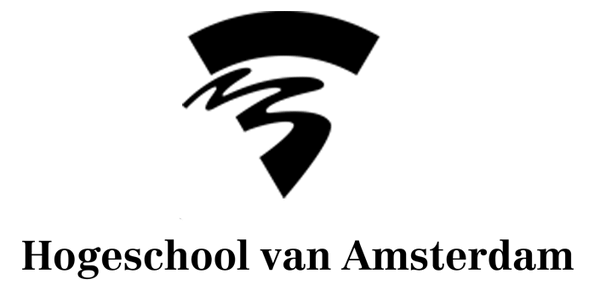
\includegraphics[width=74mm]{figures/hva-logo-png-7.png}\vspace{4em}\\
		A Preliminary Bachelor's Thesis\\
		Semester Assignment for SURF BV \\
		Department of Innovation \\
		Amsterdam University of Applied Science}
        %\vspace{3.5em}\\
		%Geophysical Institute, \\
		%University of Bergen
	%}
	\huge\date{\today}
}


%====================================================
%------------------ BEGIN DOCUMENT ------------------
%====================================================
\begin{document}
%Cause all references in bibtex file to appear in the 'References' section, even
%if they are not explicitly cite'ed in the document
%\nocite{*}

%Set the fontsize and baselineskip, if something other than 10 or 12 is required
\ifDownscaledFinalDoc
	\fontsize{\TextSize}{\BaseLineSkip}
	\selectfont
\fi

%Double line spacing for draft
\ifDraft
	\doublespacing
\fi

\renewcommand{\familydefault}{\sfdefault} %KD

%--------------------------------------------------------------------------------------------------
% FRONT MATTER
%--------------------------------------------------------------------------------------------------
\maketitle
\frontmatter
\normalfont\rmfamily
\chapter{Scientific environment (optional)}

This study is carried out at the \ldots Institute, University of Bergen. 
The work is supported by the\ldots. 
Fill this out if you are working on a project and put their logo in here. The ones below are just for example so please replace or remove them\\
%\vspace{12cm}
\vspace*{\fill}
\begin{center}
%\includegraphics[width=50mm]{figures/chess_logo_FINAL_colour_featured.png} \hspace{1cm}
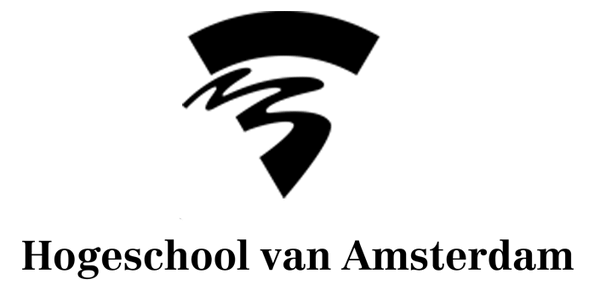
\includegraphics[width=40mm]{figures/hva-logo-png-7.png}
\hspace{1cm}


%\includegraphics[width=40mm]{figures/bjerknessenteretkvadratlogo.pdf}
\end{center}


% This is where you write the name of the subject/professional milieu involved in the study, faculty(faculties)/institute(s)/centre(s)/research groups/school of research.

% Contractual joint venture partners should also be mentioned here. If these are represented by graphic symbols (logo etc.) the it should be on this page.

% NB! Most organisations have guidelines concerning the use of their logo. These guidelines regulate who can use the logo, when the logo can be used and how. This is quite relevant when a logo is used together with information connected to other institutions/organisations. (A typical example would be rules concerning space between other written or graphic content.)

% Remember to find out which guidelines apply and ensure that they are followed!
% Most organisations will be able to provide a digital version of their logo in a suitable format.

\chapter{Acknowledgements}
%\ldots

Thank someone 


% If you want to acknowledge the people creating this template you can thank Kjersti Birkeland Daae and Stephan Kral for making it available on overleaf and Tore Birkeland and Raymond Nepstad for creating the original version of the template. 
%\vspace{5em}
\vspace*{\fill}
\begin {flushright}
Liza Darwesh\\
Amsterdam, \date{\today}
\end{flushright}
\clearpage

%quote
%\vspace*{\fill}
%\epigraph{"quotation"}{\textit{Reference}}

\chapter{Abstract}
\ldots partial- couple of sentences about motivation / task

%\include{04listofpublications}
\tableofcontents
\listoffigures
%\lstlistoflistings

%--------------------------------------------------------------------------------------------------
% MAIN MATTER
%--------------------------------------------------------------------------------------------------
\mainmatter

%
% Main chapters
%
\chapter{Introduction}
\label{chap:intro}


The introduction could be divided into subsections if this helps you organise your thoughts. It MUST include your hypotheses, though




\section{Motivation}
\label{sec:i1}
What is the general area in which you will do your work.

\section{Problem Statement}
\label{sec:i2}



\begin{figure}[htbp]
\centering
%	\includegraphics[width=12cm]{figures/somefigure} 
	\caption{caption describing the figure, if you need a figure}
	\label{fig:1}
\end{figure}


\section{Objectives}

What are your specific Hypotheses?

\section{Contribution}

What will your work add to the field? What relevance is it to the world?

\section{Thesis outline}         % Introduction
\chapter{Background}
\label{chap:thisstudy}

Could have sub sectons for dofferent theories, methods, etc. 
\section{Some theory}
Processes related to \ldots
\subsection{\ldots}
\ldots 


\begin{table}[!htbp]\centering
\def\arraystretch{1.3}
\caption{tablecaption}
\vspace{5pt}
    \arrayrulecolor{black}
    \small
\setlength{\tabcolsep}{4pt}
\begin{tabular}{lcrccccccll}
\hline
 c1 & c2 & c3 & c4 & c5 & c6 & c7 \\
\end{tabular}
\label{Tab:1}
\end{table}
\normalsize

\section{Some method}



\chapter{Methodology}
\label{chap:methodology}

\section{Design Science - if that is what you did}

\begin{table}[h!]
\begin{center}
 \begin{tabular}{||m{1em}|m{7cm}|m{7cm}||} 
 \hline
 No. & Guidelines & Compliance \\ [0.5ex] 
 \hline\hline
 1 & Design science research must produce a workable, practical artefact in the form of a construct, model, method, or instantiation & It can be used according to the original purpose, by the intended users. Be careful not to over promise. Be careful to promise the right things.\\
 \hline
 2 & Ensure that the artefact produced is relevant and important & Has anyone tried to solve it before? Why hasn't it been solved before? How important can it be? Is it too difficult?\\
 \hline
 3 & Rigorously evaluate the artefact produced & How do you know you accomplished what you wanted? Don't just ask people if they like it. Analytically using a mathematical model. Empirically using field study or experiment  \\
 \hline
 4 & Produce an artefact that makes a research contribution. & Solve a previously unsolved problem. Show that an artefact can be produced when it was previously unclear that this is possible.\\
 \hline
 5 & Follow rigorous construction methods. & The method must be rigorous and replicable  \\ 
 \hline
 6 & Show the artefact is the outcome of a search process & This is done after you're finished \\
 \hline
 7 & Clearly communicate the research process and outcome & Say a little about your thesis, any conference papers planned \\[1ex] 
 \hline
\end{tabular}
\caption{The seven guidelines for rigorous design science and how the work reported in this thesis fulfils them.}
\end{center}
\end{table}


This is an example of how you can cross reference anything marked with a label \ref{chap:intro}


\section{Experimental design}
What was your design, how did you select subjects/participants

\subsection{Threats to validity}

\section{Analytical study}

Did you derive your results through mathematical proof?
How do you know it is correct? Will it generalise to a class of problems?

\subsection{Case Study}

Did you do a case study?
\chapter{Methods}
\label{chap:methods}

What you actually did

\section{Implementation}


\section{Evaluation}
\chapter{Results and Discussion}
\label{chap:res}

This will depend entirely on what you did in \ref{chap:methods}

\section{Results and Analyses}
What did you find?


\section{Discussion}

Did your findings support your hypothesis?
Why? Why not?
\chapter{Conclusions and Future Work}
\label{chap:conc}

This Chapter concludes the thesis by summarizing the findings from the study, the contributions and possible limitations of the approach. It can also identify issues that were not solved, or new problems that came up during the work, and suggests possible directions going forward. \cite{Foldvik1985b}
%\include{3Introduction_papers}  % Introduction to the papers
%\include{4Papers}               % The papers, with cover pages
%
% Appendices
%
%\appendix
%\chapter{Some appendix}

             % Appendix A: Something

%--------------------------------------------------------------------------------------------------
% BACK MATTER
%--------------------------------------------------------------------------------------------------
\backmatter

%
% The bibliography
%

%
% Physics-style bibliography
%
%\bibliographystyle{iopart-num}

%
% Modified mathematics bibliography. Uses acm.bst
%

\bibliographystyle{agufull08}

\bibliography{Thesis}

\end{document}

